% Chapter Template

\chapter{Analysis} % Main chapter title

\label{Analysis} % Change X to a consecutive number; for referencing this chapter elsewhere, use \ref{ChapterX}

%----------------------------------------------------------------------------------------
%	SECTION 1
%----------------------------------------------------------------------------------------

The analysis results in a domain model, containing entities discovered from the requirements. These entities are obtained through a noun-analysis of the functional requirements and provides an overview of abstract concepts within the domain.\\
The communication flow between the system and its users were analyzed. This resulted in an abstract version of the API.

\section{Domain model}
\begin{figure}[H]
	\centering
	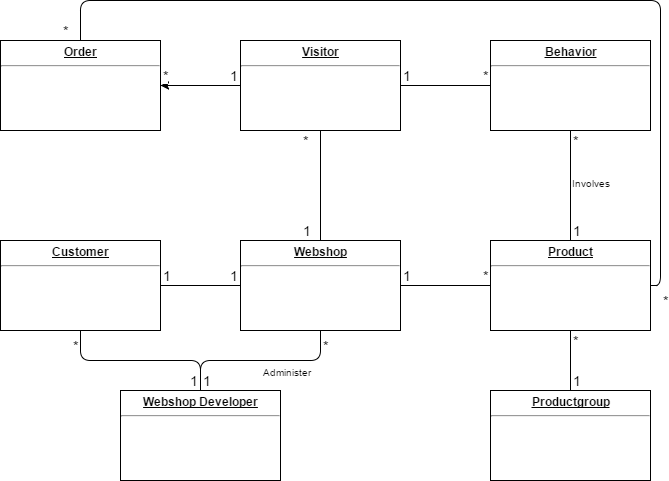
\includegraphics[width=.8\linewidth]{Figures/Domain_model.png}
	\caption{Domain model}
	\label{fig:DomainModel}
\end{figure}

The domain model in figure \ref{fig:DomainModel} is the result of the analysis of the requirements. The domain model provides an overview of concepts in the system, and how they are related.

\begin{description}
	\item[Webshop Developer] is the company developing and hosting a collection of webshops. In this project the \textit{Webshop Developer} is the company Struct A/S, who wish to add value to their services by offering product recommendations. Seen from the perspective of the project group, this is the customer who ordered a recommendation system.
	\item[Customer] is an owner of a \textit{Webshop}, developed by the \textit{Webshop Developer}. \textit{Customer} is a secondary stakeholder that desires the possibility of presenting product recommendations to its visitors.
	\item[Webshop] is the webshop owned by a \textit{Customer}, and developed and hosted by the \textit{Webshop Developer}. \textit{Webshop} offers a variety of products and presents them to the visitors of the site.
	\item[Visitor] is the end-user of the \textit{Webshop}. This is a potential customer to the owner of the \textit{Webshop} and will have product recommendations presented once the recommendation system is applied.
	\item[Product] is the different products available for purchase on the \textit{Webshop}. 
	\item[Productgroup] is the distinction between groups of products.
	\item[Behavior] describes an action of \textit{Visitor} on the \textit{Webshop}. If a \textit{Visitor} clicks on a \textit{Product}, this is considered a \textit{Behavior}. 
	\item[Order] is placed by a \textit{Visitor} resulting in a purchase of one or more \textit{Products}.
\end{description}

\section{API}
The API is essential for making the product recommendation system available to the \textit{Webshop Developer}. The following calls to the API were identified from analyzing the requirements:

\begin{description}
	\item[GetProductRecommendations] allows the client to ask for product recommendations to a \textit{Visitor}.
	\item[StoreBehavior] stores new \textit{Behavior} in the system.
	\item[DeleteBehavior] deletes existing \textit{Behavior} from the system.
	\item[StoreVisitor] stores a new \textit{Visitor} in the system.
	\item[UpdateVisitor] updates information about an existing \textit{Visitor} in the system.
	\item[DeleteVisitor] deletes an existing \textit{Visitor} from the system.
	\item[StoreProduct] stores a new \textit{Product} in the system.
	\item[UpdateProduct] updates information about an existing \textit{Product} in the system.
	\item[DeleteProduct] deletes an existing \textit{Product} from the system.
	\item[StoreOrder] stores a new \textit{Order} in the system.
	\item[DeleteOrder] deletes an existing \textit{Order} from the system.
\end{description}

The discovered API calls indicates that the system will consist of two aspects, data management and product recommendations.\\
Combining the domain model and the API calls grants an overview of the concepts and their relations within the system. 